\section{Vorlesung 21.10.2016}
\subsection{Zusammenhang}
Zusammenhang $\Rightarrow$ je zwei Konten sind durch einen \{Kanten, Weg, Pfad, Kreis\} verbunden\\
Kreis-zusammenhängend (k-zshgd) $\Rightarrow$ Pfad-zusammenhängend (p-zshgd) $\Rightarrow$ Weg-zusammenhängend (w-zshgd) $\Rightarrow$ Kantenzug-zusammenhängend (kz-zshgd)\\

\underline{Lemma}: Jeder Kantenzug zwischen x und y enthält einen Weg zwischen x und y.
\\\\
\underline{Beweis/Idee}:\\
\begin{figure}[htp]
\centering
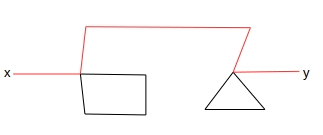
\includegraphics[scale=1.00]{lectures/161021/pix/pic1.jpg}\\
Um Weg in Pfad zu transformieren müssen Zyklen entfernt werden
\end{figure}

\underline{Lemma}: Jeder Weg zwischen x und y enthält einen Pfad (Beweis/Idee siehe vorher)
\\\\
\underline{Korollar}: Pfad-zusammenhängend (p-zshgd) $\Leftrightarrow$ Weg-zusammenhängend (w-zshgd) $\Leftrightarrow$ Kantenzug-zusammenhängend (kz-zshgd) in Zukunft einfach \textbf{zusammenhängend}\\

zusammenhängend $\nRightarrow$ Kreis-zusammenhängend
\begin{figure}[htp]
\centering
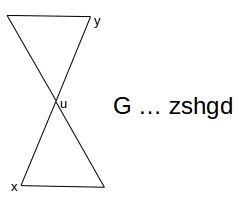
\includegraphics[scale=1.00]{lectures/161021/pix/pic2.jpg}
\end{figure}

Jeder Kantenzug von x nach y und zurück zu x muss u wenigstens 2 mal enthalten und ist deswegen kein Pfad.\\
Kreis $\equiv$ geschlossener Pfad $\Rightarrow$ $\nexists$ Kreis der x und y enthält.

\subsection{Cut-Vertex (Schnittknoten)}
Sei G ein zusammenhängender Graph. Dann ist v ein Cut vertex wenn G$\backslash$\{v\} [= Graph der entsteht wenn v und alle inzidenten\footnote{Ein Knoten v und eine Kante e heißen inzident, wenn e den Knoten v mit einem anderen Knoten verbindet} Kanten entfernt werden] in wenigstens 2 Zusammenhangs-Komponenten zerfällt.
\begin{figure}[htp]
\centering
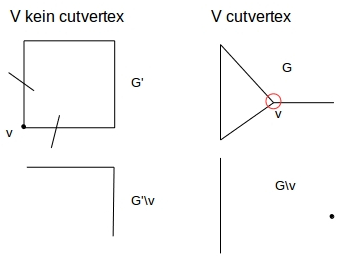
\includegraphics[scale=1.00]{lectures/161021/pix/pic3.jpg}
\end{figure}

\underline{Theorem:} Sei G ein zusammenhängender Graph mit mehr als 2 Knoten, dann seien folgende Aussagen äquivalent:\\
 - G ist Kreiszusammenhängen $\Rightarrow$ G hat keinen cut-vertex
\\\\
\underline{Beweis/Idee:}
cut-vertex $\Rightarrow$ $\neg$ Kreiszusammenhang
\begin{figure}[htp]
\centering
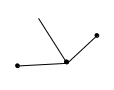
\includegraphics[scale=1.00]{lectures/161021/pix/pic4.jpg}
$|V(G)| \geq 3$
\end{figure}

\begin{figure}[htp]
\centering
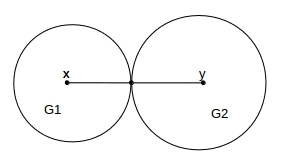
\includegraphics[scale=0.9]{lectures/161021/pix/pic5.jpg}
x in G$_1$, y in G$_2$ $\Rightarrow$ $\nexists$ Kreis durch x und y $\Rightarrow$ $\neg$ Kreiszusammenhang
\end{figure}

\newpage
\underline{zu 2.:}\\
Kreiszusammenhang $\Rightarrow$ $\nexists$ cut-vertex ($|V(G)| \geq 3$)\\
Kreiszusammenhang $\Rightarrow$ $\exists$ mindestens 2 disjunkte Wege von x nach y, d.h. es gibt keinen Knoten durch den alle Wege von x nach y gehen $\Rightarrow$ es kann keinen cut-vertex geben
\\\\
\underline{Spezialfälle:}\\
\begin{enumerate}
	\item $|V(G)| = 1$ (nur ein Knoten) $\Rightarrow$ zusammenhängend, $\neg$ Kreiszusammenhängen, kein cut-vertex
	\item $|V(G)| = 2$ (zwei Knoten, eine Kante) $\Rightarrow$ zusammenhängend, $\neg$ Kreiszusammenhängen, kein cut-vertex
\end{enumerate}

\underline{Definition.:} Ein Graph G ist 2-zusammenhängend wenn G$\backslash$v für alle $v \in V(G)$ zusammenhängend und nicht ein einzelner Knoten oder leer ist $\Leftrightarrow$ G$\backslash$v zusammenhängend und enthält wenigstens 1 Kante\\

Spezialfälle 1 und 2 sind zusammenhängend aber nicht 2-zusammenhängend
\\\\
G ist 2-zusammenhängend $\Leftrightarrow$ G enthält keinen cut-vertex
\begin{figure}[htp]
\centering
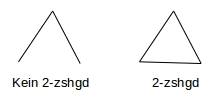
\includegraphics[scale=0.9]{lectures/161021/pix/pic6.jpg}
\end{figure}

Sei $W \subseteq V(G)$ und G$\backslash$W der Graph der aus G ensteht, wenn alle Knoten in W und deren inzidenten Kanten entfernt werden.
\\\\
G ist k-zusammenhängend, wenn G$\backslash$W für alle W mit $|W| = k-1$ zusammenhängend und weder K$_1$ noch leer ist.
\begin{figure}[htp]
\centering
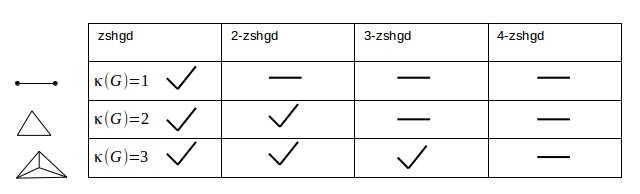
\includegraphics[scale=1]{lectures/161021/pix/pic7.jpg}
\end{figure}

\underline{Definition:} $\kappa (G)$ ist die größte Zahl k sodass G k-zusammenhängend $\Leftrightarrow$ G ist k-zusammenhängend aber nicht (k+1)-zusammenhängend
\\\\
$\kappa(G)$ heißt die Konnektivität von G
\begin{figure}[htp]
\centering
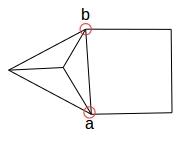
\includegraphics[scale=1]{lectures/161021/pix/pic8.jpg}
\end{figure}

\underline{Bemerkung:} G ist k-zusammenhängend $\Rightarrow$ G$\backslash$v ist (k-1)-zusammenhängend für alle v$\in$V(G)

\newpage
\subsection{Spezielle Graphen}

\underline{vollständige Graphen:}
\begin{figure}[htp]
\centering
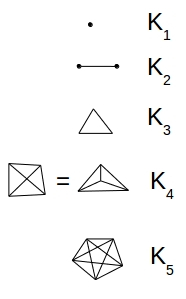
\includegraphics[scale=1]{lectures/161021/pix/pic9.jpg}
$K_n … n=V(K_n)$ Knoten, $\binom{n}{2}$ Kanten
\end{figure}

\underline{Kreise:}
\begin{figure}[htp]
\centering
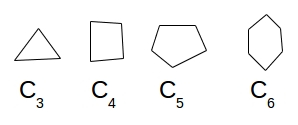
\includegraphics[scale=1]{lectures/161021/pix/pic10.jpg}
\end{figure}

\underline{Baum:} zusammenhängender Graph der keine Kreise enthält\\
\underline{Wald:} disjunkte Vereinigung von Bäumen $\Leftrightarrow$ kreisfreier Graph\\
\underline{Teilgraphen:} H(W,F) ist Teilgraph von G(V,E) wenn
\begin{enumerate}
	\item W $\subseteq$ V
	\item F $\subseteq$ E
	\item \{x,y\} $\in$ F $\Rightarrow$ x,y $\in$ W
\end{enumerate}

\underline{Induzierter Teilgraph:} H ist induzierter Teilgraph von wenn
\begin{enumerate}
	\item H Teilgraph von G
	\item x,y $\in$ W und \{x,y\} $\in$ E $\Rightarrow$ \{x,y\} $\in$ F
\end{enumerate}

\underline{spannende Teilgraphen (spanning subgraphs):} Teilgraphen W=V
\\\\
\underline{Spannbäume (spanning trees):} Teilbaum von G, der alle Knoten enthält\\
jeder zusammenhängende Graph hat einen Spannbaum

\subsection{algebraische Graphentheorie}
\textbf{Idee:} Graphen $\Rightarrow$ Matrizen $\Rightarrow$ Eigensch. der Matrizen $\Rightarrow$ Eigensch. der Graphen
\subsubsection{Matrizendarstellung von Graphen}
Adjezenz-Matrix A $\rightarrow$ fixe Reihenfolge der Knoten (x $<$ y)\\
$A_{xyy}=
	\begin{cases}
		\text{1 wenn x,y benachbart} \{x,y\} \in E\\
		\text{0 sonst}
	\end{cases}
$

\underline{Beispiel:}\\
\begin{figure}[htp]
\centering
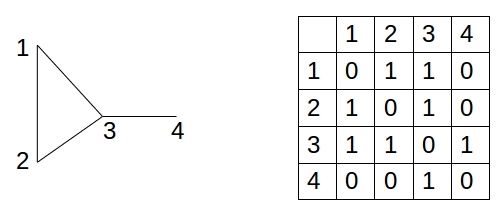
\includegraphics[scale=1]{lectures/161021/pix/pic11.jpg}
\end{figure}

\underline{Eigenschaften von A:}
\begin{itemize}
	\item symetrisch
	\item für simple Graphen A$_{xx}$=0 für alle A
	\item für unterschiedlich Nummerierungen unterschiedliche A-Matrizen
\end{itemize}

\subsubsection{Permutationsmatrix}
quadratische Matrix P sodass in jeder Zeile und jeder Spalte genau eine 1 steht und sonst 0 (P=(p$_{ij}$))
\\\\
\textbf{Satz:} zwei Graphen mit Adjazenz-Matritzen A und B sind isomorph genau dann wenn es eine P gibt sodass A$\cdot$P=P$\cdot$B
\\\\
PP$^T$=P$^T$P=I ($\widehat{=}$ Einheitsmatrix) [... mit P$^T_{ij}$=P$_{ji}$]\\
$A \cdot P = P \cdot B$\\
$A \cdot \underbrace{PP^T}_{I}=P \cdot B \cdot P^T$
\\\\
Zwei quadratische Matrizen A,B heißen ähnlich wenn es einer invertierbare Matrix Q gibt, sodass $A \cdot Q = Q \cdot B$
\\\\
\textbf{Satz:} ähnliche Matrizen haben das gleiche \underline{Spektrum}
\begin{figure}[htp]
\centering
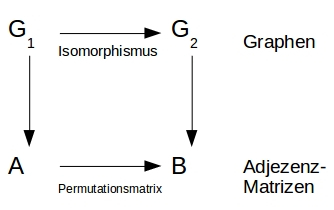
\includegraphics[scale=1]{lectures/161021/pix/pic12.jpg}
\end{figure}

j=$\pi(i)$\\
P$_{ij}$=1\\
P$_{ij'}$=0 für j'$\neq$j\\
P$_{i'j}$=0 für i'$\neq$i\\
\\\\
\underline{Beispiel:}
\begin{figure}[htp]
\centering
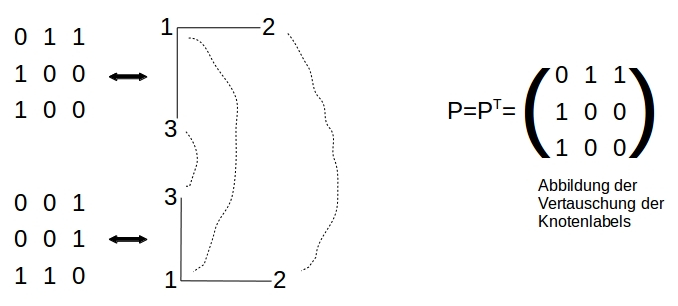
\includegraphics[width=1\textwidth]{lectures/161021/pix/pic13.jpg}
\end{figure}

\newpage
\subsection{Spektrum einer Matrix}
- für unsere Fälle quadratisch\\
- Eigenvektor x und Eigenwerte $\lambda$ von A erfüllen $A \cdot x = \lambda \cdot x$
\\\\
Eine nxn-Matrix hat höchstens n verschiedene Eigenwerte
\begin{itemize}
	\item wenn A symetrisch (A=A$^T$) sind alle Eigenwerte reell
	\item es gibt $det(A-\lambda \cdot I)=0$ $\rightarrow$ liefert Gleichung n-ten Grades für $\lambda$
\end{itemize}

\underline{Bemerkung:} $det(A) = \displaystyle \sum_{\pi \in S_n} a_{1 \pi (1)} \cdot a_{2 \pi (2)} \cdot ... a_{n \pi (n)} \cdot (-1)^{sgn(\pi)}$\\
\underline{Definition:} Das Spektrum einer Matrix ist die Menge der Eigenwerte\\
Graph $\rightarrow$ Adjazenz-Matrix $\rightarrow$ Spektrum der Adjazenz-Matrix
\\\\
\textbf{Satz:} das Spektrum einer A-Matrix ist eine Graphinvariante einer Graphenklasse